\documentclass[%
  hyperref={%
    colorlinks,
    linkcolor=sDarkBlue,
    urlcolor=sDarkBlue,
    citecolor=sDarkBlue
  },
  aspectratio=169
]{beamer}
\usetheme{sakura}
\ltjsetparameter{%
  jacharrange={%
    -2,  % Exclude Greek and Cyrillic letters.
    -3,  % Punctuations and Miscellaneous symbols.
    -7   % Hangul
  }
}
\usepackage{luatexja-ruby}
\usepackage{breakurl}
\usepackage{booktabs}
\usepackage{ccicons}
\usepackage{subcaption}
\usepackage{fontawesome5}
\usepackage{amsmath,amssymb}
\usepackage{framed}
\usepackage{listings}
\usepackage{tikz}
\usepackage{pgfplots}
\usepackage{tikz-dependency}
\usepackage{wtref}
\usepackage{polyglossia}
\setdefaultlanguage{japanese}
\setotherlanguage[variant=polytonic]{greek}
\setotherlanguage{russian}
\setotherlanguage[variant=modern]{korean}
\setotherlanguage{thai}
\setotherlanguage{vietnamese}
\setotherlanguage{english}
\renewcommand{\tablename}{表}
\renewcommand{\figurename}{図}
\newcounter{ngloss}
\renewcommand{\thengloss}{\alph{ngloss}}
\makeatletter
\newenvironment{gloss}[1][]{
  \refstepcounter{ngloss}
  \begin{table}[#1]
  \raggedright
}{
  \end{table}
}
\makeatother
\newref{tab}
\setrefstyle{tab}{prefix=表}
\newref{gloss}
\setrefstyle{gloss}{refcmd=グロス(\ref{#1})}
\newref{fig}
\setrefstyle{fig}{prefix=図}
\newref{math}
\setrefstyle{math}{refcmd=式(\ref{#1})}
\setbeamertemplate{caption}[numbered]
\setbeamertemplate{caption label separator}{:}
\setbeamertemplate{itemize items}[circle]
\setbeamertemplate{bibliography item}{\insertbiblabel}
\usetikzlibrary{automata,positioning,arrows,calc}
\usepackage[%
  backend=biber,
  style=pecorarista,
  natbib=true,
  maxnames=2,
  language=auto
]{biblatex}
\addbibresource{demo.bib}
\DeclareMathOperator{\exponential}{exp}
\newcommand\header[1]{\multicolumn{1}{c}{\textbf{#1}}}
\newenvironment{quoteblock}{%
  \def\FrameCommand{%
    {\color{sLightGray}{\vrule width 3pt}}%
      \hspace{10pt}
  }%
  \MakeFramed {\advance\hsize-\width \FrameRestore}}%
{\endMakeFramed}
% For inline codes
\lstnewenvironment{LaTeXCode}{%
  \lstset{%
    language={[LaTeX]TeX},
    escapechar={|},
    alsoletter={*},
    basicstyle=\ttfamily\footnotesize,
    commentstyle=\color{sDarkBlue},
    texcsstyle=*\color{sRed}\bfseries,
    moretexcs={%
      usebeamertemplate,
      newref,
      setrefstyle,
      mathlabel,
      mathref,
      ltjsetparameter,
      arabicfont,
      newfontfamily,
      translitfont,
      SetTranslitFont,
      SetTranslitStyle,
      SetTranslitConvention,
      RequireBibliographyStyle,
      AtEveryBibitem,
      DeclareNameAlias,
      DeclareFieldFormat,
      printlist,
      printdate,
      addcomma,
      addperiod,
      finentry,
      revsdnamepunct,
      renewbibmacro*,
      renewcommand*,
      iffieldequalstr,
    }
  }
}{}
\lstnewenvironment{PythonCode}{%
  \lstset{%
    basicstyle=\ttfamily\footnotesize,
    keywordstyle=\color{sRed}\bfseries,
    morekeywords={def, with, as, for, in}
  }
}{}
\renewcommand\refname{参考文献}
\renewcommand\appendixname{付録}
\title{Lua\TeX{}-jaとbeamerで研究発表用のスライドを作る}
\institute{所属}
\author{著者 太郎}
\date{{\number\year}年{\number\month}月{\number\day}日}
% https://tex.stackexchange.com/questions/2541/beamer-frame-numbering-in-appendix
\newcommand{\backupbegin}{
   \newcounter{framenumberappendix}
   \setcounter{framenumberappendix}{\value{framenumber}}
}
\newcommand{\backupend}{
   \addtocounter{framenumberappendix}{-\value{framenumber}}
   \addtocounter{framenumber}{\value{framenumberappendix}}
}
\begin{document}

    \maketitle

    \section{はじめに}
    \begin{frame}
        \frametitle{はじめに}
        このスライドは \faGithub\ \href{https://github.com/pecorarista/sakuratheme}{\ttfamily pecorarista/sakuratheme}のデモとして作ったものです.

        \bigskip

        そのため作り方を詳しく説明することはしませんが,
        コードはすべて上記のレポジトリに含まれているので気になる方は参照ください.
    \end{frame}

    \begin{frame}[fragile]
        \frametitle{用紙サイズ}
        アスペクト比の設定は\texttt{documentclass}のオプションで設定することができます.
        デフォルトは4:3です.
        \begin{leftbar}
\begin{LaTeXCode}
\documentclass[%
    aspectratio=169
]{beamer}
\end{LaTeXCode}
        \end{leftbar}
    \end{frame}

    \section{Tips}
    \begin{frame}
        \frametitle{表の挿入}
        Beamerでは論文中の表のソースコードをほぼそのまま利用できて便利です.
        \begin{table}
            \centering
            \caption{表の例.}\tablabel{tab}
            \begin{tabular}{lrrr}
                \toprule
                \header{Model}   & \header{Precision} & \header{Recall} & \header{F1} \\
                \midrule
                \texttt{model-a} & 0.75 & 0.60 & 0.67 \\
                \texttt{model-b} & \textbf{0.80} & 0.70 & 0.75 \\
                \texttt{model-c} & 0.65 & \textbf{0.85} & 0.74 \\
                \texttt{model-d} & 0.78 & 0.78 & \textbf{0.78} \\
                \bottomrule
            \end{tabular}
        \end{table}
    \end{frame}

    \begin{frame}
        \frametitle{アイコン}
        アイコンを入力したい場合は\href{https://ctan.org/pkg/fontawesome5?lang=en}{fontawesome5}パッケージを利用すると便利です.
        \begin{table}
            \centering
            \caption{アイコンを使った表の例.}\tablabel{tabfontawesome}
            \begin{tabular}{lcc}
                \toprule
                \header{Model}   & \header{Algorithm A} & \header{Algorithm B} \\
                \midrule
                \texttt{model-a} & \textcolor{sRed}{\faTimes} & \textcolor{sRed}{\faTimes} \\
                \texttt{model-b} & \textcolor{sRed}{\faTimes} & \textcolor{sOKGreen}{\faCheck} \\
                \texttt{model-c} & \textcolor{sOKGreen}{\faCheck} & \textcolor{sRed}{\faTimes} \\
                \texttt{model-d} & \textcolor{sOKGreen}{\faCheck} & \textcolor{sOKGreen}{\faCheck} \\
                \bottomrule
            \end{tabular}
        \end{table}
    \end{frame}

    \begin{frame}[fragile]
        \frametitle{CCアイコン}
        Creative Commonsライセンスの作品を引用する際には\href{https://ctan.org/pkg/ccicons}{\texttt{ccicons}}パッケージのアイコンを利用すると便利です.

        \bigskip

        \begin{figure}
            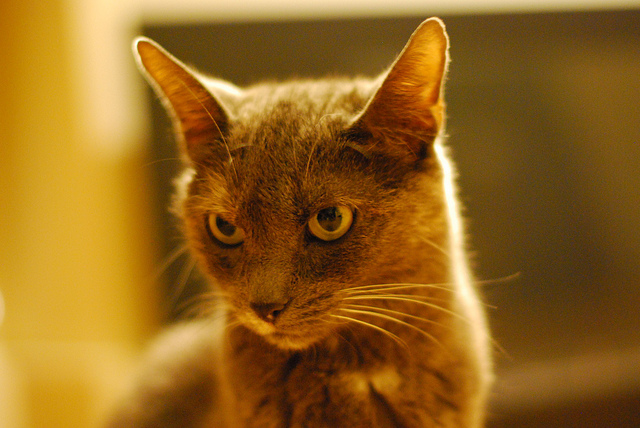
\includegraphics[width=0.4\textwidth]{figures/cat.jpg}
            \caption{\href{https://www.flickr.com/photos/selda_eigler/8687127864/in/photolist-eeDNsC-qWFs4R-7CNDjJ-9c8DxY-eeDNhC-UCZ63T-dJNGUc-e5Nk39-988EVA-kUgwo-owDcVP-jQGjjt-5zkGTy-7WRCUo-b91XbZ-Mj8Ku-5pzwSA-9Bct2H-7CNHMY-7CJJMB-8MyEYn-9x45Mp-7JTq8M-ZrpGJ9-8fRht4-4SxVZT-5pzwjJ-ZsPJjL-aE44GL-dF6uWD-kqbHgM-5F373J-ZsQrVG-qyD7E9-ajyDPL-4WDvTp-KbDSc-5kCxD9-4MdeUo-pgDQcG-pPWrXD-662AFD-oTnC8k-apYceQ-nJSaaY-7CJLZv-7CJJMn-7CNFsU-XNMWkw-ccdtT9}{\emph{Cat} by Selda Eigler} \ccby.}
        \end{figure}

    \end{frame}


    \begin{frame}[fragile]
        \frametitle{箇条書き}
        \settowidth{\leftmargini}{\usebeamertemplate{itemize item}}
        \addtolength{\leftmargini}{\labelsep}
        箇条書きのインデントを下げたくない場合はフレーム内で
        \begin{leftbar}
\begin{LaTeXCode}
\settowidth{\leftmargini}{\usebeamertemplate{itemize item}}
\addtolength{\leftmargini}{\labelsep}
\end{LaTeXCode}
        \end{leftbar}
        としてください.

        \bigskip

        以下のようになります:

        \smallskip

        \begin{itemize}
            \item \begin{korean}금연\end{korean}
            \item \begin{thai}
ห้ามสูบบุหรี่
            \end{thai}
            \item \begin{vietnamese}
Cấm hút thuốc
            \end{vietnamese}
        \end{itemize}

    \end{frame}


    \begin{frame}[fragile]
        \frametitle{コード}
        \href{https://ctan.org/pkg/listings?lang=en}{\texttt{listing}}パッケージを使って
        コードを挿入することができます.その際にフレームに\texttt{fragile}オプションを指定しないと,
        タイプセットの際にエラーが生じるので気をつけてください.

        \bigskip

        左の縦線は\href{https://ctan.org/pkg/framed}{\texttt{framed}}パッケージの\texttt{leftbar}環境を使っています.

        \smallskip

    \begin{leftbar}
\begin{PythonCode}
def main() -> None:
    with Path('test.jsonl').open(mode='r') as r:
        reader = jsonlines.Reader(r)
        for obj in reader:
            tokens = tokenize(obj['text'])
\end{PythonCode}
    \end{leftbar}

    \end{frame}

    \begin{frame}
        \frametitle{長め文章の引用}
        左の縦線は長めの文章を引用する際にも便利です.

        \bigskip

        \begin{quoteblock}

        \begin{greek}[variant=ancient]
    ἅπαν δὲ ὄνομά ἐστιν ἢ κύριον ἢ γλῶττα ἢ μεταφορὰ ἢ κόσμος ἢ πεποιημένον ἢ ἐπεκτεταμένον ἢ ὑφῃρημένον ἢ ἐξηλλαγμένον.
        \end{greek}

            \hfill \citetitle{poetics}
        \end{quoteblock}

        \begin{quoteblock}
            「あの森\ruby{琴}{ライラ}の宿でせう。
            あたしきつとあの森の中には、
            むかしの大きなオーケストラの人たちが集まつていらつしやると思ふわ。
            まはりには青い孔雀やなんかたくさんゐると思ふわ。」
            女の子が答へました。

            \hfill \citetitle{ginga}
        \end{quoteblock}
    \end{frame}


    \begin{frame}[fragile]
        \frametitle{グロス}
        大量に記載するのでなければ\href{https://ctan.org/pkg/gb4e?lang=en}{gb4e}ではなく\texttt{table}環境で十分だと思います.

        \bigskip

        \begin{gloss}
            \raggedright
            \begin{tabular}{lllll}
                (a) & {Это} & {учебник} & {русского} & {языка} \\
                % {Э'то} {уче'бник} {ру'сского} {языка'} \\
                    & {èto} & {učebnik} & {russk-ovo} & {jazyk-a} \\
                    & {this} & {textbook.\textsc{sg.nom}} & {Russian-\textsc{m.sg.gen}} & {language-\textsc{gen}} \\
                    & \multicolumn{4}{l}{``This is a textbook of the Russian language.''}
            \end{tabular}
            \glosslabel{ru}
        \end{gloss}

        \bigskip

        上の\glossref{ru}は\texttt{table}環境(をラップして定義した\texttt{gloss}環境)で作成しています.
        詳しくはこのスライドのソースコードを参照してください.
    \end{frame}

    \begin{frame}[fragile]
    \frametitle{アラビア文字I}
        もしアラビア文字を入力したければ\href{https://ctan.org/pkg/arabluatex?lang=en}{arabluatex}の利用をおすすめします.
    \begin{leftbar}
\begin{LaTeXCode}
\usepackage{arabluatex}
\newfontfamily\arabicfont[%
  Script=Arabic, % enable ligatures
  RawFeature={%
    +anum, % use eastern arabic numerals
    +ss05} % put kasrah below shadda
]{Fira GO}
\newfontfamily\translitfont[Ligatures=TeX]{%
  TeX Gyre Termes
}
\SetTranslitFont{\translitfont}
\SetTranslitStyle{\itshape} % \upshape, \itshape
\SetTranslitConvention{arabica} % dmg, loc, arabica
\end{LaTeXCode}
    \end{leftbar}
    \end{frame}

    \begin{frame}[fragile]
        \frametitle{アラビア文字II}
        ラテン文字で入力できるのでRTL(右から左への横書き)や合字に対応していないエディタでも編集できます.
        転写の方法は\texttt{dmg}, \texttt{arabica}, \texttt{loc}の3種類から選べます.

        \begin{leftbar}
\begin{LaTeXCode}
\begin{arab}[fullvoc]
    'anta tatakallamu 'l-lu.gaTa
    'l-`arabiyyaTa jayyidaN!
\end{arab}
\arb[trans]{'anta tatakallamu
            'l-lu.gaTa 'l-`arabiyyaTa jayyidaN!}
\end{LaTeXCode}
        \end{leftbar}

        \begin{arab}[fullvoc]
            'anta tatakallamu 'l-lu.gaTa 'l-`arabiyyaTa jayyidaN!
        \end{arab}

        \bigskip

        \arb[trans]{'anta tatakallamu 'l-lu.gaTa 'l-`arabiyyaTa jayyidaN!}
    \end{frame}

    \begin{frame}
        \frametitle{複数の図の挿入}
        複数の図を挿入するには\href{https://ctan.org/pkg/subcaption}{\texttt{subcaption}}を利用します.

        \bigskip

        \begin{figure}
            \begin{subfigure}[t]{0.38\textwidth}
                \centering
                \scalebox{.9}{%
                    \begin{dependency}[hide label]
                        \begin{deptext}[column sep=2\zw]
                            兵庫を \& 訪れた。 \\
                        \end{deptext}
                        \depedge{2}{1}{目的語}
                    \end{dependency}
                }
                \caption{文節単位・ラベルなし}\figlabel{dep-without-labels}
            \end{subfigure}
            \begin{subfigure}[t]{0.6\textwidth}
                \centering
                \scalebox{.9}{%
                    \begin{dependency}[text only label,label style={above}]
                        \begin{deptext}[column sep=2\zw]
                            兵庫  \& を  \& 訪れ \& た。 \\
                            {\scriptsize 固有名詞} \& {\scriptsize 接置詞} \& {\scriptsize 動詞} \& {\scriptsize 助動詞} \\
                        \end{deptext}
                        \depedge{1}{2}{格表示}
                        \depedge{3}{1}{目的語}
                        \depedge{3}{4}{助動詞}
                    \end{dependency}
                }
                \caption{単語単位・ラベルあり}\figlabel{dep-with-labels}
            \end{subfigure}
            \caption{文「兵庫を訪れた。」を係り受け解析し,図示したもの.}
        \end{figure}
        \figref{dep-without-labels}や\figref{dep-with-labels}のように参照することができます.
    \end{frame}

    \begin{frame}[fragile]
        \frametitle{ページの分割}
        \texttt{columns}環境を使うことでページを垂直に分割することができます。

        \smallskip

        \begin{columns}[onlytextwidth]

            \begin{column}{0.48\textwidth}
                \begin{quoteblock}
                    la biz e lə sɔlɛ\textsuperscript{j} sə dispytɛ~‖
                    \ ʃak\~{ɛ} asyʁ\~{ɑ} kilɛtɛ lə ply f\"{ɔ}ʁ̞~‖
                    \ k\~{ɑ}t ilz\~{ɔ} vy \~{ɛ} vwɑjaʒœ ki sav\~{ɑ}sɛ~‖
                    \ \~{ɑ}vlope d\~{ɑ} s\~{ɔ} m\~{ɑ}to~‖
                    \ iː s\~{ɔ} t\~{ɔ}be dak\"{ɔ}ʁ̥ kə səlɥi ki aʁivʁe
                    ləpʁ̥əmje a lə lɥi fɛʁote~‖
                    səʁə ʁəgaʁde k\"{ɔ}m lə ply f\"{ɔ}ʁ̞~‖
\ al\"{ɔ}ʁ̞
la biz sɛ̝
miz a sufle də tut se f\"{ɔ}ʁ̞s~‖
                    \ mɛ ply ɛl suflɛ ply lə vwɑjaʒœʁ̞
                    sɛʁɛ s\~{ɔ} m\~{ɑ}totʊʁ̞
                    də lɥi~‖
                    \ …

                    \hfill \textit{French in \citetitle{ipa}}
                \end{quoteblock}

            \end{column}

            \begin{column}{0.48\textwidth}

                IPAの入力は\href{https://github.com/samhocevar/wincompose}{WinCompose}
                を使うと楽になります:
                \begin{itemize}
                    \item \texttt{[Compose]} + \texttt{o} + \texttt{e} \ \ltjjachar`→\ œ
                    \item \texttt{[Compose]} + \texttt{h} + \texttt{r} \ \ltjjachar`→\ ʁ
                \end{itemize}

                \bigskip

                装飾的な記号は \LaTeX のコマンドを使うと編集画面で見やすいです:

                \begin{itemize}
                    \item \texttt{\textcolor{sRed}{\bfseries \textbackslash\textasciitilde}\{o\}} \ \ltjjachar`→\ \~{o}
                    \item \texttt{k\textcolor{sRed}{\bfseries \textbackslash textsuperscript}\{j\}} \ \ltjjachar`→\ k\textsuperscript{j}
                \end{itemize}

            \end{column}

        \end{columns}
    \end{frame}

    \begin{frame}[fragile]
        \frametitle{参考文献の設定}
        \href{https://ctan.org/pkg/biblatex?lang=en}{\texttt{biblatex}}を使います。
        文献情報が単純な場合は\texttt{chicago-notes}をベースに\texttt{.bbx}を
        以下のような修正を行うことで日本語対応ができます。
        \begin{leftbar}
\begin{LaTeXCode}
\RequireBibliographyStyle{chicago-notes}

\AtEveryBibitem{%
  \iffieldequalstr{langid}{japanese}{%
    \DeclareNameAlias{sortname}{family-given}
    \DeclareFieldFormat{title}{『|{{\ttfamily\bfseries \textcolor{sXlsxGreen}{\#1}}}|』}
    \renewcommand*{\revsdnamepunct}{}
    \renewcommand*{\addperiod}{}
    \renewcommand*{\addcomma}{}
    \renewcommand*{\finentry}{.}
    \renewbibmacro*{publ+loc+year}{%
      \printlist{publisher}(\printdate).
    }}{}
}
\end{LaTeXCode}
        \end{leftbar}
    \end{frame}


    \begin{frame}
        \frametitle{その他}
        箇条書きの項目が鉤括弧から始まるときの注意点
        \begin{itemize}
            \item こんにちは
            \item 「こんにちは」

                行頭の余白が大きい
            \item \leavevmode\inhibitglue 「こんにちは」

                \texttt{\textbackslash item \textbackslash leavevmode\textbackslash inhibitglue} で余白を調整
        \end{itemize}

        \bigskip

        参照:\href{http://doratex.hatenablog.jp/entry/20140714/1405302796}{「TeX Live 2014のpTeX系列における\textbackslash inhibitglueの仕様変更」}
    \end{frame}

    \backupbegin

    \begin{frame}[%
        % allowframebreaks,  % Enable `allowframebreaks` if the number of pages is larger than 1.
        plain
    ]{参考文献}

    \begin{english}
    \printbibliography[%
        title={参考文献}  % for PDF bookmark
    ]
    \end{english}

    \end{frame}

    \backupend

\end{document}
